\documentclass[12pt]{article}
\usepackage[english]{babel}
\usepackage{natbib}
\usepackage{url}
\usepackage[utf8x]{inputenc}
\usepackage{amsmath}
\usepackage{graphicx}
\graphicspath{{images/}}
\usepackage{parskip}
\usepackage{fancyhdr}
\usepackage{vmargin}
\setmarginsrb{3 cm}{2.5 cm}{3 cm}{2.5 cm}{1 cm}{1.5 cm}{1 cm}{1.5 cm}

\title{Evolution of Modern Healthcare}								% Title
\author{21111038}								% Author
\date{3 Feb 2022}											% Date

\makeatletter
\let\thetitle\@title
\let\theauthor\@author
\let\thedate\@date
\makeatother

\pagestyle{fancy}
\fancyhf{}
\rhead{\theauthor}
\lhead{\thetitle}
\cfoot{\thepage}

\begin{document}

%%%%%%%%%%%%%%%%%%%%%%%%%%%%%%%%%%%%%%%%%%%%%%%%%%%%%%%%%%%%%%%%%%%%%%%%%%%%%%%%%%%%%%%%%

\begin{titlepage}
	\centering
    \vspace*{0.5 cm}
    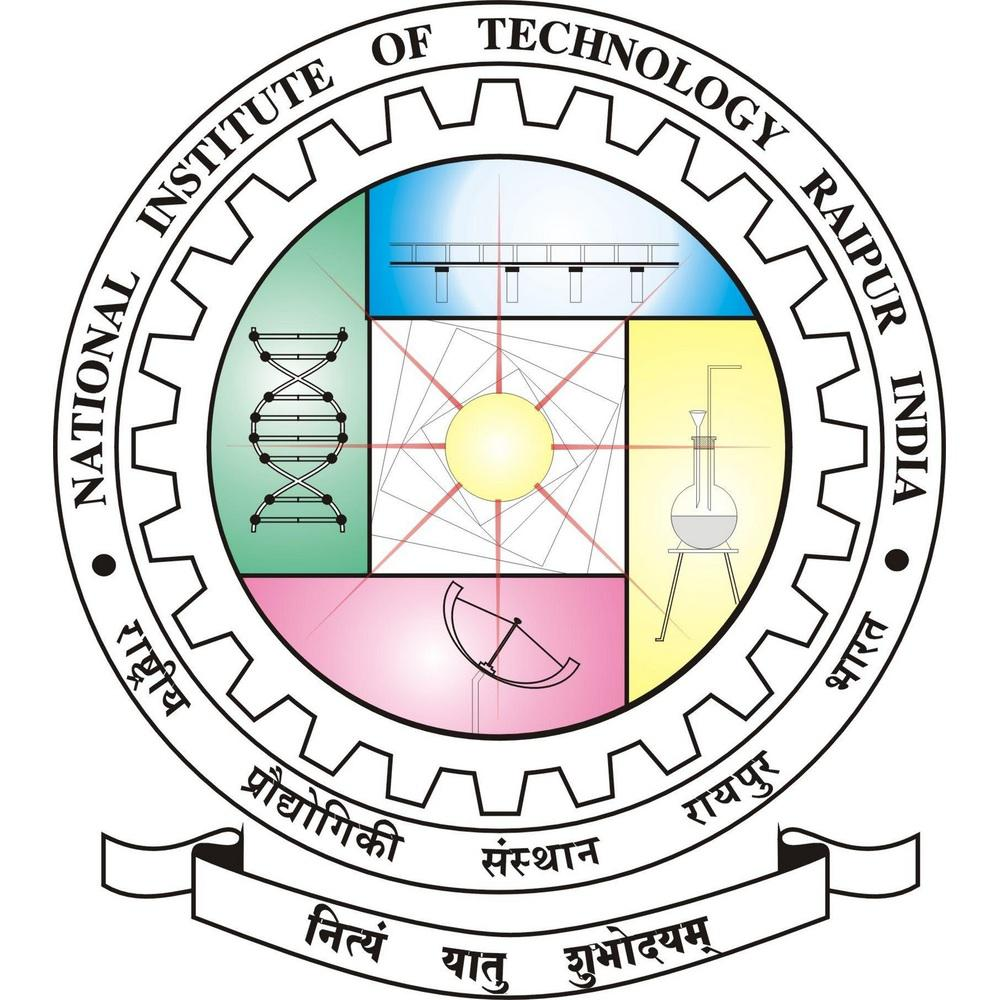
\includegraphics[scale = 0.20]{logo.jpg}\\[1.0 cm]	% University Logo
    \textsc{\LARGE  National Institute of Technology\newline\newline Raipur}\\[2.0 cm]	% University Name
	\textsc{\Large assignment 02}\\[0.5 cm]				% Course Code
	\rule{\linewidth}{0.2 mm} \\[0.4 cm]
	{ \huge \bfseries \thetitle}\\
	\rule{\linewidth}{0.2 mm} \\[1.5 cm]
	
	\begin{minipage}{0.4\textwidth}
		\begin{flushleft} \large
			\emph{Submitted To:}\\
			Saurabh Gupta\\
            Asst. Professor\\
            Department of Biomedical Engineering\\
			\end{flushleft}
			\end{minipage}~
			\begin{minipage}{0.4\textwidth}
            
			\begin{flushright} \large
			\emph{Submitted By :} \\
			Pradnya Manmode\\
            21111038\\
        First Semester\\
        Biomedical Engineering\\
		\end{flushright}
        
	\end{minipage}\\[2 cm]
	
	
    
    
    
    
	
\end{titlepage}


\title{ASSIGNMENT 02}
\maketitle

\indent

A health system, also known as health care system or healthcare system, is the organization of people, institutions, and resources that deliver health care services to meet the health needs of target populations.
\\
There is a wide variety of health systems around the world, with as many histories and organizational structures as there are nations. Implicitly, nations must design and develop health systems in accordance with their needs and resources, although common elements in virtually all health systems are primary healthcare and public health measures. 
\\
The 20th century witnessed many truly revolutionary advances in health care. Increasingly, discoveries in the biological sciences are being applied toward the development of medicines and treatments targeted to refined subsets of patients to better address genetic or life circumstances.
\\

In today’s complex clinical environment, contending with the challenges and realizing the yet untapped potential of technological and biomedical research innovations will require a sharper focus on the evidence as a way to drive improvements in the effectiveness and efficiency of the healthcare system. 

\indent
Health systems have evolved significantly with technology throughout the years, with each innovation aiming to reach a higher level of transformation, efficiency, and interoperability than the last. Nowadays, we are seeing a shift toward Real-Time Health Systems (RTHS), in which relevant data is being shared in real-time between devices, people, and workflows.

These systems are shaping the new era of health care by driving better outcomes for patients, care teams, hospital administrators, and facility staff. But how does a hospital enable a real-time health system? And how do these new technologies differ from earlier hospital technology? In this blog, we explore the evolution of the real-time health system that has led to the use of Digital Twin technology today. 
\\
New computer technology such as desktop computers to enter, and local servers to store data laid the foundation for the first Electronic Medical Records (EMR) system, developed in the early 1970s.  The traditional EMR system is a digital version of a patient’s charts. Patient data is stored on an internal server, containing patient medical history, diagnoses, medications, consults, orders, laboratory test results, and more. The goal of an EMR is to enable faster and easier access to more accurate patient information for clinicians.
\\
Fast-forward to the Smart Hospital Digital Twin - a technology that achieves a seamless interconnected real-time health system. Digital Twins have evolved rapidly over the past few years. Smart Hospital Digital Twins connect previously disparate systems to give clinicians and patients an overview of the bigger picture. Unlike other solutions, Digital Twins present a holistic approach, looking at the entire hospital environment combining data from various subsystems to provide new insights in real-time, based on the interactions between people, processes, and connected things.
\\
Information rich overviews not only offers actionable insights for the present, but also unlocks insights into the past and future states of the hospital; unlocking historic trend analysis and real time alert and responsive for time-critical situations. For instance, through Thought Wire’s Early Warning application, the capturing and transcription of vital signs have been streamlined leveraging mobile devices. This critical data is automatically transcribed to the EMR and computed through a Digital-Twin powered algorithm which calculates the patient’s current state, generating a “score” for the potential risk of a code blue event. Previously, vitals were often written on ‘shadow documentation’ like paper and only later entered into an EMR system. The latency of data transcription into the EMR could be addressed with automatic entry into an EMR, however this alone is not able to capture the benefit of pro-actively using the data for preventative care. With the Early Warning app, the real-time entry and analysis is what enables healthcare providers to take immediate action, preventing code blue events before they can occur.
\\
The healthcare system has improve a lot due to new technologies.
\\
We should keep improving the health system for us. 

 



\end{document}